\documentclass{article}
\usepackage[utf8]{inputenc}

% Page setup
\usepackage[a4paper,landscape,margin=2cm]{geometry}
\usepackage{amsmath}

% Typography
\usepackage[scaled]{helvet}
\let\familydefault\sfdefault

\usepackage[usenames,svgnames]{xcolor}
\usepackage{tikz,pgfplots}
\usetikzlibrary{positioning,arrows,intersections,calc}

\definecolor{colorwhite}      {RGB}{255,255,255}
\definecolor{colorblack}      {RGB}{  0,  0,  0}
\definecolor{colorweb}        {RGB}{200,200,200}
\definecolor{colorqueue}      {RGB}{120,122,234}
\definecolor{colortriples}    {RGB}{245, 66, 66}
\definecolor{colordocuments}  {RGB}{ 79,142,209}
\definecolor{colorlinks}      {RGB}{143,232,046}
\definecolor{colorextractors} {RGB}{199,212,104}

\begin{document}
\pagestyle{empty}
\tikzset{>=latex}
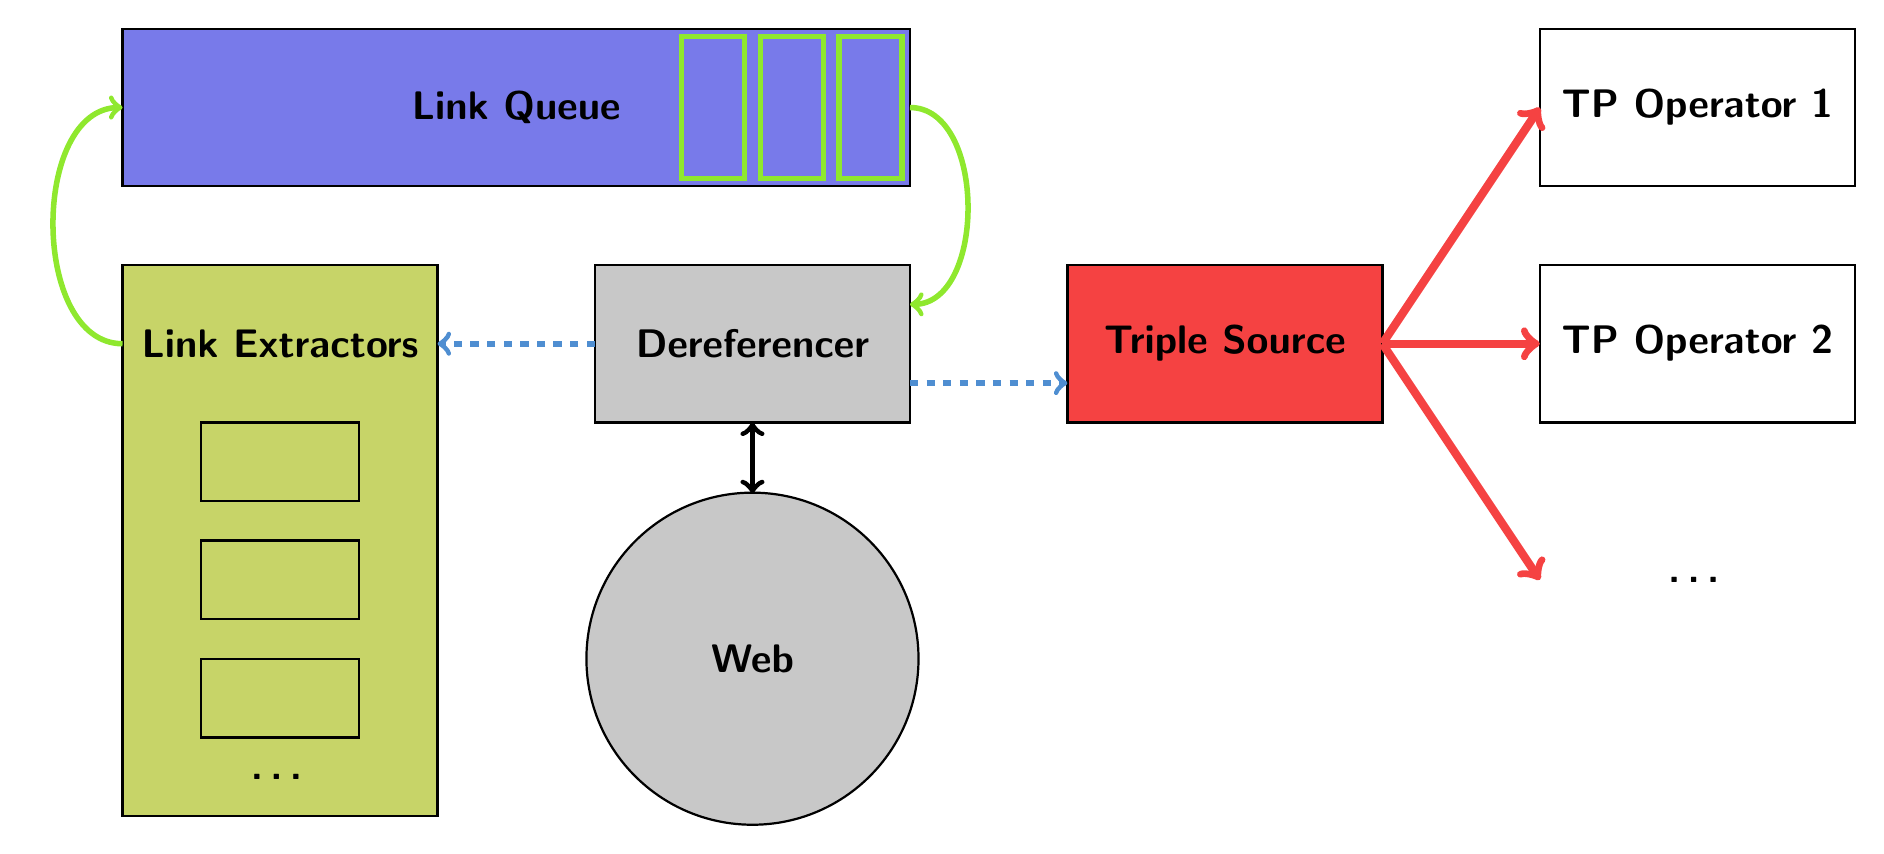
\begin{tikzpicture}[
    node distance = 10em, auto, thick,
    title2/.style={text=colortext,font={\Large\itshape}},
    title/.style={text=colorblack,font={\Large\bfseries}},
    code/.style={text=colortext,font={}},
    key/.style={text=colortext,font={\small\itshape}},
    triples/.style={colortriples,line width=3pt},
    documents/.style={colordocuments,line width=2pt,dashed},
    data/.style={colorblack,line width=2pt},
    links/.style={colorlinks,line width=2pt},
]


    % Web
    \draw[fill=colorweb] (0,0) circle (60pt);
    \node[title] at (0,0) (web) {Web};
    
    % Dereferencer
    \draw[fill=colorweb] (-2,3) rectangle (2,5);
    \node[title] at (0,4) (dereferencer) {Dereferencer};
    
    % Link Queue
    \draw[fill=colorqueue] (-8,6) rectangle (2,8);
    \node[title] at (-3,7) (queue) {Link Queue};
    \draw[links] (1.1,6.1) rectangle (1.9,7.9);
    \draw[links] (0.1,6.1) rectangle (0.9,7.9);
    \draw[links] (-0.1,6.1) rectangle (-0.9,7.9);
    
    % Link Extractors
    \draw[fill=colorextractors] (-8,-2) rectangle (-4,5);
    \node[title] at (-6,4) (extractors) {Link Extractors};
    \draw[fill=colorextractors] (-7,3) rectangle (-5,2);
    \draw[fill=colorextractors] (-7,1.5) rectangle (-5,0.5);
    \draw[fill=colorextractors] (-7,0) rectangle (-5,-1);
    \node[title] at (-6,-1.5) {\ldots};
    
    % Triple Source
    \draw[fill=colortriples] (4,3) rectangle (8,5);
    \node[title] at (6,4) (source) {Triple Source};
    
    % Query Operators
    \draw[fill=colorwhite] (10,6) rectangle (14,8);
    \node[title] at (12,7) (operator1) {TP Operator 1};
    \draw[fill=colorwhite] (10,3) rectangle (14,5);
    \node[title] at (12,4) (operator2) {TP Operator 2};
    \node[title] at (12,1) (operator3) {\ldots};
    
    % Arrows
    \draw[->,links] (2,7) to [out=0,in=0] (2,4.5); % queue to dereferencer
    \draw[<->,data] (0,3) to (0,2.1); % dereferencer to web
    \draw[->,documents] (-2,4) to (-4,4); % dereferencer to link extractors
    \draw[->,documents] (2,3.5) to (4,3.5); % dereferencer to source
    \draw[->,links] (-8,4) to [out=180,in=180] (-8,7); % extractors to queue
    \draw[->,triples] (8,4) to (10,7); % source to tp1
    \draw[->,triples] (8,4) to (10,4); % source to tp2
    \draw[->,triples] (8,4) to (10,1); % source to tp3
    

    % Person Alice
    %\draw[fill=colorperson] (2,4) circle (30pt);
    %\node[person] at (2,4) (alice) {Alice};

    % Person Dave
    %\draw[fill=colorperson] (17,4) circle (30pt);
    %\node[person] at (17,4) (dave) {Dave};

    % Pod Alice
    %\draw[fill=colorpod] (5.5,0) rectangle (13.5,5.5);
    %\node[title,text width=10em] at (7.5,5) {Pod Alice};
    %\node[code,text width=10em] at (11.5,5) {https://alice.pods.org/};
    %
    %% Address Book Alice
    %\draw[fill=colorbook] (6,0.5) rectangle (13,4);
    %\node[title,text width=10em] at (8,3.5) {Address Book};
    %\node[code,text width=10em] at (13,3.5) {/contacts};
    %\node[code,text width=20em] at (9.8,2) {$<$/profile\#me$>$ :knows\\
    %\ \ $<$https://bob.pods.org/profile\#me$>$,\\
    %\ \ $<$https://carol.org/\#i$>$,\\
    %\ldots};
    %
    %% Pod Bob
    %\draw[fill=colorpod] (0,-6.5) rectangle (8,-1.5);
    %\node[title,text width=10em] at (2,-2) {Pod Bob};
    %\node[code,text width=10em] at (6,-2) {https://bob.pods.org/};
    %
    %% Profile Bob
    %\draw[fill=colorbook] (0.5,-6) rectangle (7.5,-3);
    %\node[title,text width=10em] at (2.5,-3.5) {Profile};
    %\node[code,text width=10em] at (7.5,-3.5) {/profile};
    %\node[code,text width=20em] at (4.3,-5) {$<$/profile\#me$>$ :name "Bob".\\
    %$<$/profile\#me$>$ :email $<$bob@mail.org$>$.\\
    %$<$/profile\#me$>$ :telephone "0499 12 34 56".};
    %%\node[key] at (4,-6.25) {Alice $\in$ S$_F$; Dave $\in$ S$_E$};
    %
    %% Pod Carol
    %\draw[fill=colorpod] (11,-6.5) rectangle (19,-1.5);
    %\node[title,text width=10em] at (13,-2) {Pod Carol};
    %\node[code,text width=10em] at (17.7,-2) {https://carol.org/};
    %
    %% Profile Carol
    %\draw[fill=colorbook] (11.5,-6) rectangle (18.5,-3);
    %\node[title,text width=10em] at (13.5,-3.5) {Profile};
    %\node[code,text width=10em] at (19,-3.5) {/};
    %\node[code,text width=20em] at (15.3,-5) {$<$/\#i$>$ :name "Carol".\\
    %$<$/\#i$>$ :email $<$i@carol.org$>$.\\
    %$<$/\#i$>$ :telephone "0499 11 22 33".};
   %% \node[key] at (15,-6.25) {Alice $\in$ S$_A$; Dave $\in$ S$_E$};
    %
    %% Arrows between pods
    %\draw[->,thick,dashed](6.6,2.2) to [out=180,in=90] (4,-3);
    %\draw[->,thick,dashed](10,1.75) to [out=0,in=90] (15,-3);

    % Arrows from people to data
    %\draw[->,thick,colorperson] (alice) -- (6,3.5);
    %\draw[->,thick,colorperson] (alice) -- (3.5,-3);
    %\draw[->,thick,colorperson] (alice) -- (11.5,-3);
    %\draw[->,thick,colorperson] (dave)  -- (13,3.5);
    %\draw[->,thick,colorperson] (dave)  -- (7.5,-3);
    %\draw[->,thick,colorperson] (dave)  -- (15.5,-3);

\end{tikzpicture}
\end{document}
